\subsubsection{Parallelization Aspects}

%%%%%%%%%%%%%%%%%%%%%%%%%%%%%%%%%%%%%%%%%%%%%%%%%%%%%%%%%%

\begin{frame}[t]{Parallelization Aspects}
\small

\vspace{-5mm}
\begin{columns}
	\begin{column}{0.5\textwidth}
		\begin{figure}
			\centering
			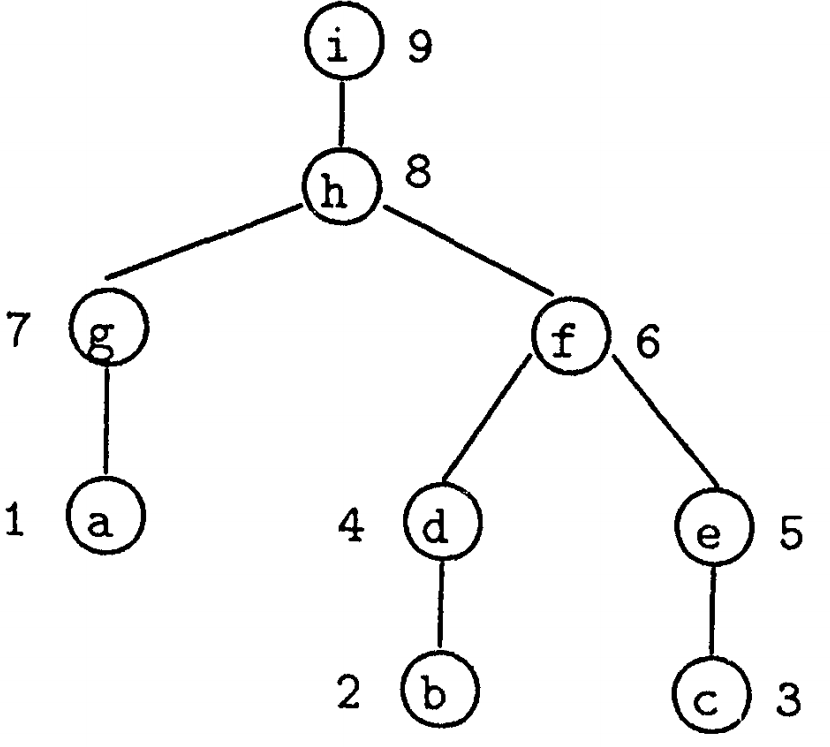
\includegraphics[width=0.3\textheight]{figures/chapter-2/elimination-tree-mm.png}
			\caption{Original elimination tree}
		\end{figure}
	\end{column}
	
	\begin{column}{0.5\textwidth}
		\begin{figure}
			\centering
			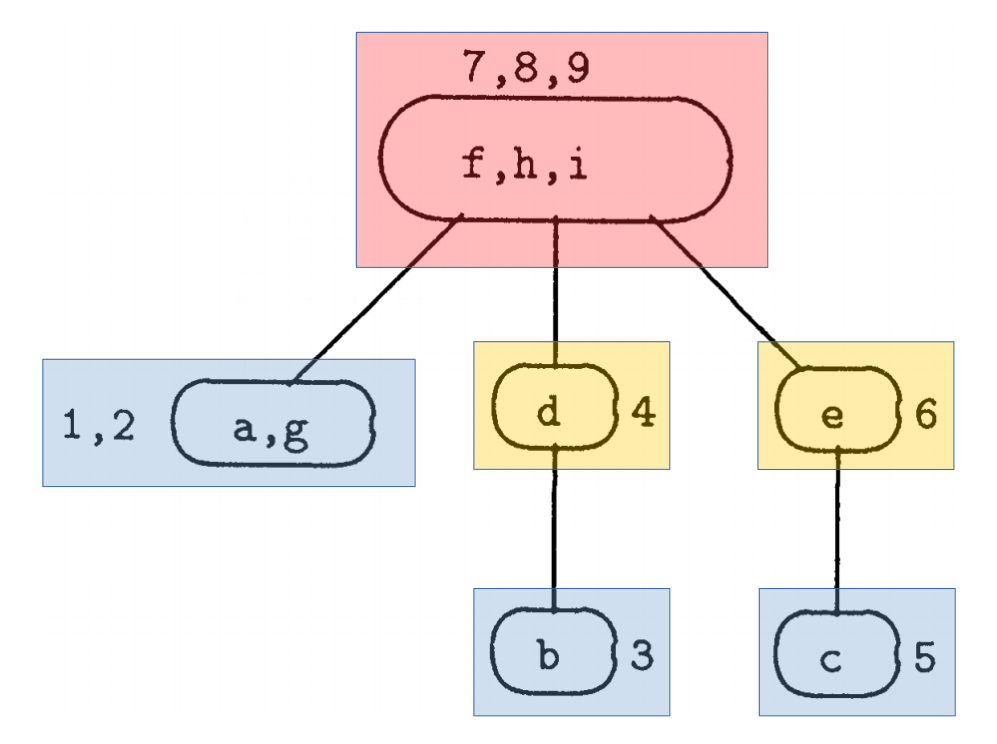
\includegraphics[width=0.6\textwidth]{figures/chapter-2/elimination-tree-parallel.png}
			\caption{Supernodal/assembly tree}
		\end{figure}
	\end{column}
	
\end{columns}

\begin{figure}[!htpb]
	\centering
	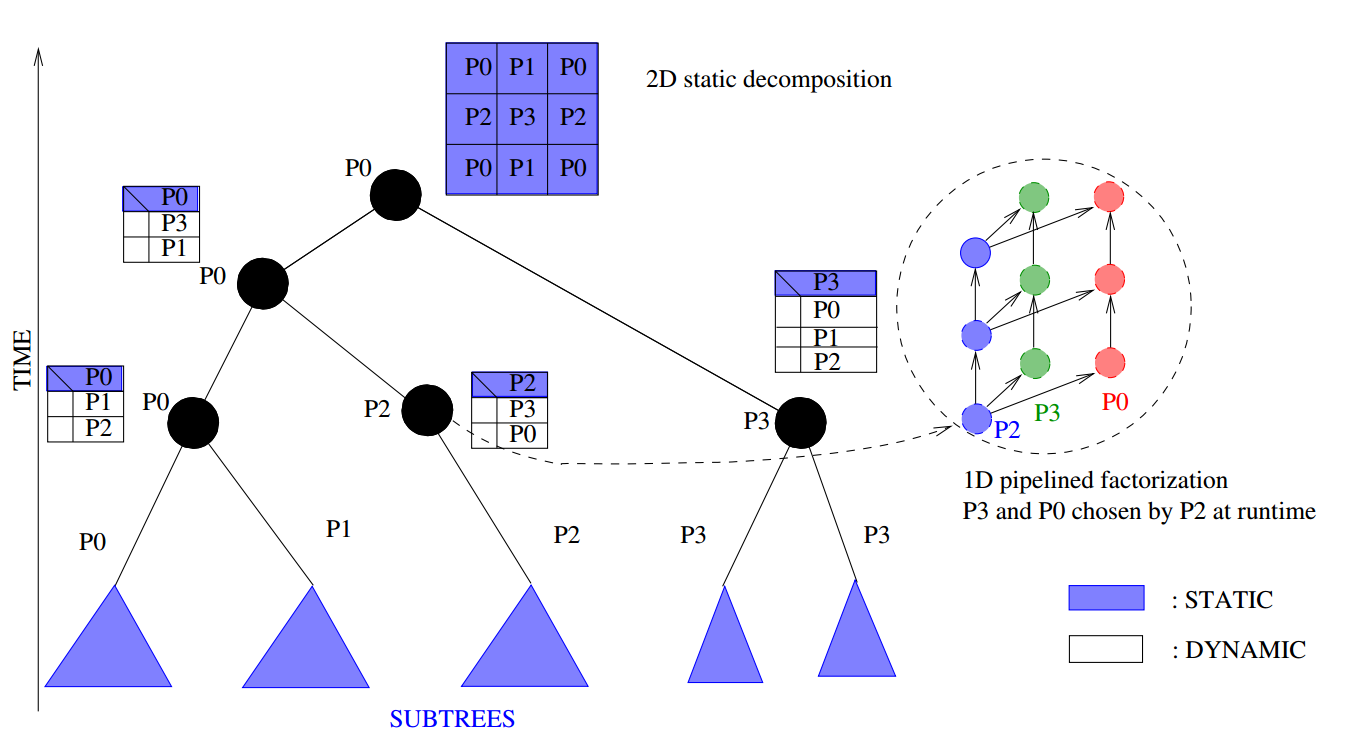
\includegraphics[width=0.55\textwidth]{figures/chapter-2/mumps-task-data-parallelism-2.png}
	\caption{Static and dynamic scheduling in MUMPS, \cite{l2012multifrontal}}
	\label{fig:mumps:mapping-and-scheduling}
\end{figure}

\end{frame}
